\section{Adaptive Noise Cancellation}

\begin{enumerate}[label=\alph*), leftmargin=*]

%% a)
\item
%

Let the pure sine wave $x(n)$, the noisy signal $s(n)$, the noise term $\eta(n)$ and the ALE filter output $\hat{x}(n; \Delta)$, parametrised by the delay parameter $\Delta$.
Then the Mean Squared Error (MSE) is given by:

\begin{align}
    \mathtt{MSE} =
    \E \bigg[ \big( s(n) - \hat{x}(n; \Delta) \big)^{2} \bigg]  &=  \E \bigg[ \big( x(n) + \eta(n) - \hat{x}(n; \Delta) \big)^{2} \bigg] \\
                                                                &=  \E \bigg[ \big( \eta(n) + (x(n) - \hat{x}(n; \Delta)) \big)^{2} \bigg] \\
                                                                &=  \E \bigg[ \eta^{2}(n) \bigg] +
                                                                    \E \bigg[ \big( x(n) - \hat{x}(n; \Delta) \big)^{2} \bigg] +
                                                                   2\E \bigg[ \eta(n) \big(x(n) - \hat{x}(n; \Delta) \big) \bigg]
\label{eq:ale_mse}
\end{align}

The first term, noise power $\E [ \eta^{2}(n) ]$, is independent of $\Delta$, while the second term, Mean Squared Prediction Error $\E [ (x(n) - \hat{x}(n; \Delta))^{2} ]$ is not
a function of noise $\eta(n)$. Hence, the last term only involves both the delay $\Delta$ (through $\hat{x}(n)$) and the noise term, so we will minimise it:

\begin{equation}
    \underset{\Delta \in \sN}{min}\ \E \bigg[ \eta(n) \big(x(n) - \hat{x}(n; \Delta) \big) \bigg]
\end{equation}

Using the fact that $x(n)$ and $\eta(n)$ are uncorrelated the term $\E [ \eta(n) x(n) ]$ vanished:

\begin{align}
    \underset{\Delta \in \sN}{min}\ \E \bigg[ \eta(n) \hat{x}(n; \Delta) \bigg] &\rightarrow
        \underset{\Delta \in \sN}{min}\ \E \bigg[ \big( u(n) + 0.5u(n-2) \big) \vw^{T} \vu(n; \Delta) \bigg] \\
                                                                                &\rightarrow
        \underset{\Delta \in \sN}{min}\ \E \bigg[ \big( u(n) + 0.5u(n-2) \big) \sum_{i=0}^{M-1} w_{i} s(n - \Delta - i) \bigg] \\
                                                                                &\rightarrow
        \underset{\Delta \in \sN}{min}\ \E \bigg[ \big( u(n) + 0.5u(n-2) \big) \sum_{i=0}^{M-1} w_{i} \big( x(n - \Delta - i) + \eta(n - \Delta - i) \big) \bigg] \\
                                                                                &\rightarrow
        \underset{\Delta \in \sN}{min}\ \E \bigg[ \big( u(n) + 0.5u(n-2) \big) \sum_{i=0}^{M-1} w_{i} \big( \eta(n - \Delta - i) \big) \bigg] \\
                                                                                &\rightarrow
        \underset{\Delta \in \sN}{min}\ \E \bigg[ \big( u(n) + 0.5u(n-2) \big) \sum_{i=0}^{M-1} w_{i} \big( u(n - \Delta - i) + 0.5 u(n - 2 - \Delta - i) \big) \bigg]
\label{con:delta} \\
                                                                                &\rightarrow
        0, \quad \Delta > 2
\end{align}

Since $u(n)$ is identically and \textbf{independently} distributed white noise:

\begin{equation}
    \E \bigg[ u(n) u(n - j) \bigg] = 0, \quad \forall j \neq 0
\end{equation}

therefore the expectation in (\ref{con:delta}) is zero and thus minimised for $\Delta > 2$, since the terms are non time-overlapping.
This is an expected result, since the colored noise signal $\eta(n)$ is a second order MA process.

The theoretical optimal delay range, $\Delta > 2$ is also verified empirically. In figure \ref{fig:3_3_a_1} the clean signal $x(n)$ against, $s(n)$ and filter output $\hat{x}(n)$
are illustrated for different delay $\Delta$ values. Moreover, the MPSE as a function of $\Delta$ is also plotted in figure \ref{fig:3_3_a_2}, verifying the improved performance $\Delta > 2$.
All experiments are conducted using a fixed model order $M = 5$ LMS filter.

\begin{figure}[h]
    \centering
    \begin{subfigure}{0.49\textwidth}
        \centering
        \includegraphics[height=1.5in]{report/adaptive-signal-processing/adaptive-noise-cancellation/assets/a/ale_overlay-Delta_1}
    \end{subfigure}
    ~
    \begin{subfigure}{0.49\textwidth}
        \centering
        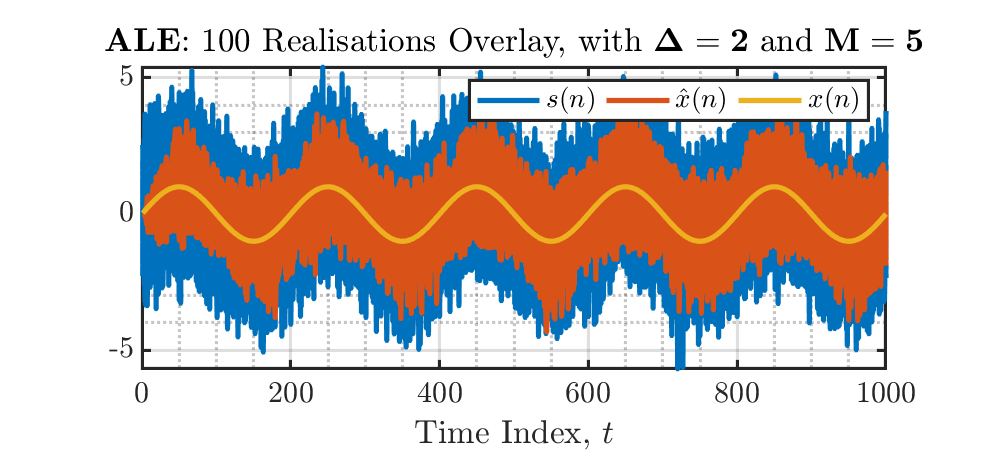
\includegraphics[height=1.5in]{report/adaptive-signal-processing/adaptive-noise-cancellation/assets/a/ale_overlay-Delta_2}
    \end{subfigure}
    ~
    ~
    \begin{subfigure}{0.49\textwidth}
        \centering
        \includegraphics[height=1.5in]{report/adaptive-signal-processing/adaptive-noise-cancellation/assets/a/ale_overlay-Delta_3}
    \end{subfigure}
    ~
    \begin{subfigure}{0.49\textwidth}
        \centering
        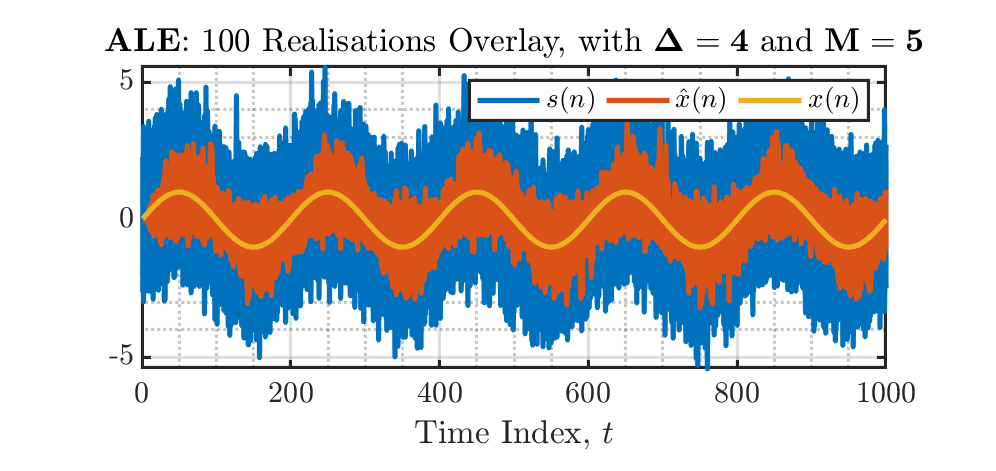
\includegraphics[height=1.5in]{report/adaptive-signal-processing/adaptive-noise-cancellation/assets/a/ale_overlay-Delta_4}
    \end{subfigure}
    \caption{ALE: overlay plots for various $\Delta$ delays, for fixed $M=5$.}
    \label{fig:3_3_a_1}
\end{figure}

\begin{figure}[h]
    \centering
    \begin{subfigure}{0.49\textwidth}
        \centering
        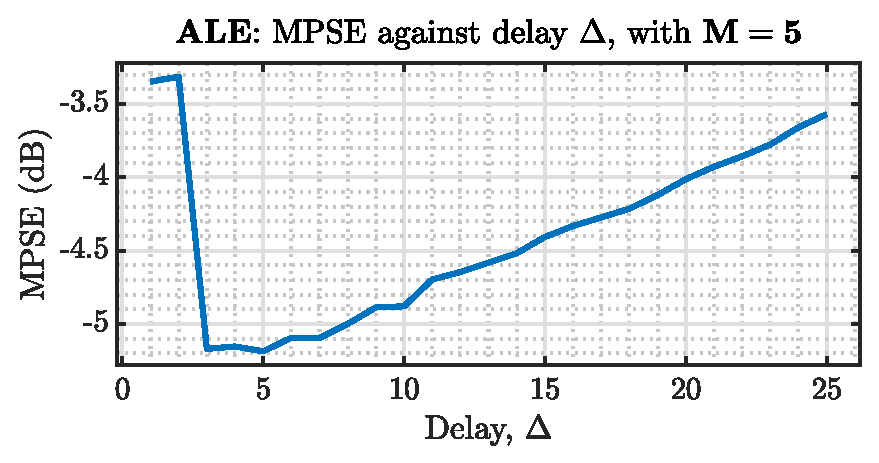
\includegraphics[height=1.5in]{report/adaptive-signal-processing/adaptive-noise-cancellation/assets/a/ale_mpse}
    \end{subfigure}
    \caption{ALE: MPSE against $\Delta$, for fixed $M=5$.}
    \label{fig:3_3_a_2}
\end{figure}

%% b)
\item
%

The experiments are repeated varying now both the delay parameter, $\Delta$, and the model order, $M$, obtaining figures \ref{fig:3_3_b_1}, \ref{fig:3_3_b_2}.
We notice that the mean squared prediction error (MPSE) is minimised for the hyperparmeters pair $(\Delta, M) = (3, 6)$.

Over-modelling (large $M$) results in excess degrees of freedom that increase computational complexity and over-fit noise, degrading
model performance. For model order $M=6$ MPSE is minimised, while the model complutational load is still not prohibitive.

In the previous part we showed theoretically that for $\Delta > 2$ the noise and the filter output are uncorrelated thus MSE is minimised.
Nonetheless, the second term in (\ref{eq:ale_mse}) was ignored. The impact of this term on the MPSE is illustrated in figure \ref{fig:3_3_b_2},
where very large $\Delta$ (i.e $\Delta = 25$) inevitably cause a time-shift between the filter output $\hat{x}(n)$ and the true sine wave $x(n)$.
Hence, $\Delta = 3$ is the optimal parameter, minimising delay effects between $x(n)$ and $\hat{x}(n)$, as well as guaranteeing uncorrelation between
$\hat{x}(n)$ and $\eta(n)$.

\begin{figure}[h]
    \centering
    \begin{subfigure}{0.49\textwidth}
        \centering
        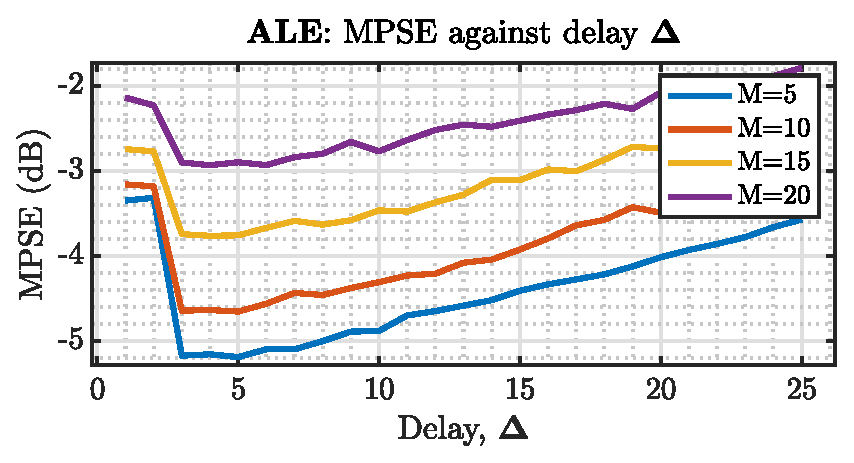
\includegraphics[height=1.5in]{report/adaptive-signal-processing/adaptive-noise-cancellation/assets/b/ale_mpse_vs_Delta}
    \end{subfigure}
    ~
    \begin{subfigure}{0.49\textwidth}
        \centering
        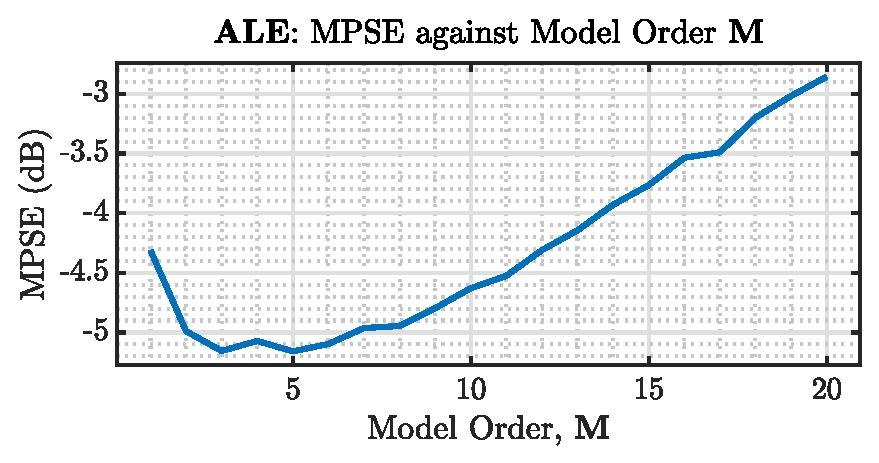
\includegraphics[height=1.5in]{report/adaptive-signal-processing/adaptive-noise-cancellation/assets/b/ale_mpse_vs_M}
    \end{subfigure}
    \caption{ALE: MPSE against delay $\Delta$ and model order $M$.}
    \label{fig:3_3_b_1}
\end{figure}

\begin{figure}[h]
    \centering
    \begin{subfigure}{0.32\textwidth}
        \centering
        \includegraphics[height=1in]{report/adaptive-signal-processing/adaptive-noise-cancellation/assets/b/ale_overlay-Delta_1}
    \end{subfigure}
    ~ 
    \begin{subfigure}{0.32\textwidth}
        \centering
        \includegraphics[height=1in]{report/adaptive-signal-processing/adaptive-noise-cancellation/assets/b/ale_overlay-Delta_3}
    \end{subfigure}
    ~
    \begin{subfigure}{0.32\textwidth}
        \centering
        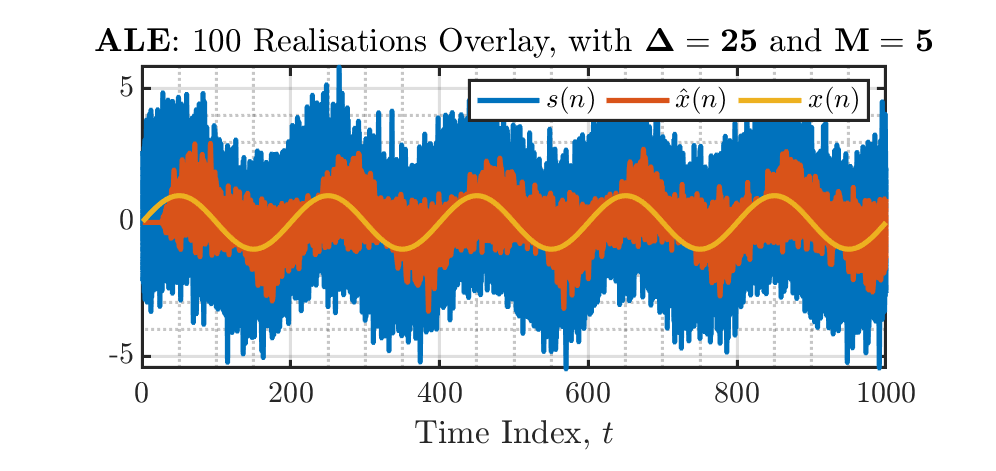
\includegraphics[height=1in]{report/adaptive-signal-processing/adaptive-noise-cancellation/assets/b/ale_overlay-Delta_25}
    \end{subfigure}
    \caption{ALE: model deterioration for large delays $\Delta$.}
    \label{fig:3_3_b_2}
\end{figure}

%% c)
\item
%

We compare the performance of the Adaptive Noise Cancellation (ANC) configuration to the Adaptive Line Enchancer (ALE) configuration, used in previous parts.
The colored noise $\epsilon(n)$ is used as input to the LMS filter to perform ANC, such that:

\begin{equation}
    \epsilon(n) = 0.9 \eta(n) + 0.05 
\end{equation}

and as a result $\epsilon(n)$ is the secondary noise signal, correlated to the $\eta(n)$, primary noise signal. Note that the relationship between the two signals
is unknown to the ANC algorithm.

\begin{figure}[h]
    \centering
    \begin{subfigure}{0.49\textwidth}
        \centering
        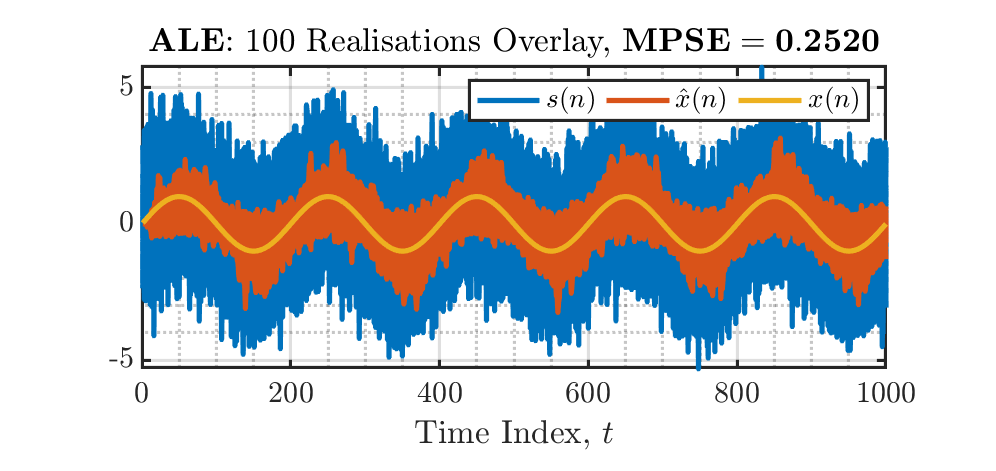
\includegraphics[height=1.5in]{report/adaptive-signal-processing/adaptive-noise-cancellation/assets/c/ALE_overlay}
    \end{subfigure}
    ~
    \begin{subfigure}{0.49\textwidth}
        \centering
        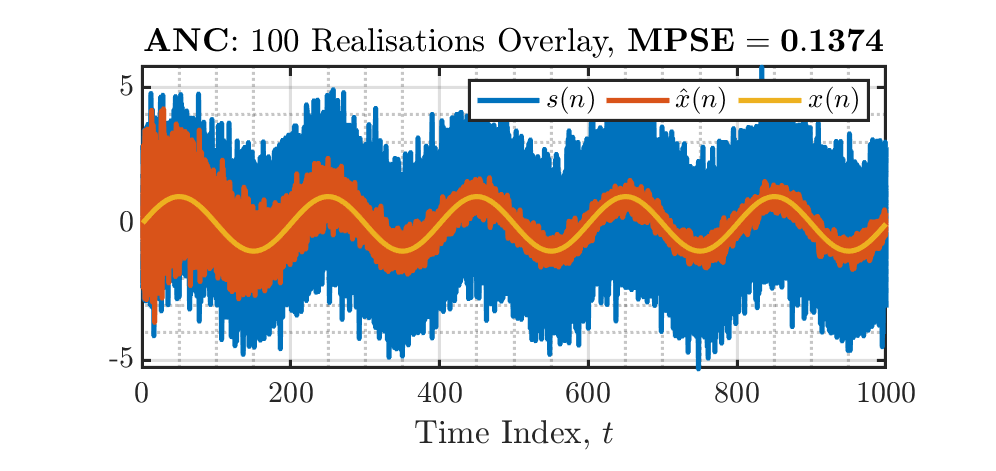
\includegraphics[height=1.5in]{report/adaptive-signal-processing/adaptive-noise-cancellation/assets/c/ANC_overlay}
    \end{subfigure}
    \caption{ALE vs ANC: overlay plots and mean prediction squared error.}
    \label{fig:3_3_c_1}
\end{figure}

In figure \ref{fig:3_3_c_1} the overlay plots for 100 realisations of the process $x(n)$ are provided, along with the denoised versions of both the ALE and ANC configurations.
ANC performs overall better, with MPSE = 0.1374, than the ALE configuration, which scores MPSE = 0.2520. Nonetheless, we highlight the fact that the ANC algorithm
does poorly in the first timesteps, but for $t > 400$, it tracks the true signal $x(n)$ much better. An ensemble of realisations of the process is also simulated and its mean are illustrated in figure \ref{fig:3_3_c_2}.

\begin{figure}[h]
    \centering
    \begin{subfigure}{0.49\textwidth}
        \centering
        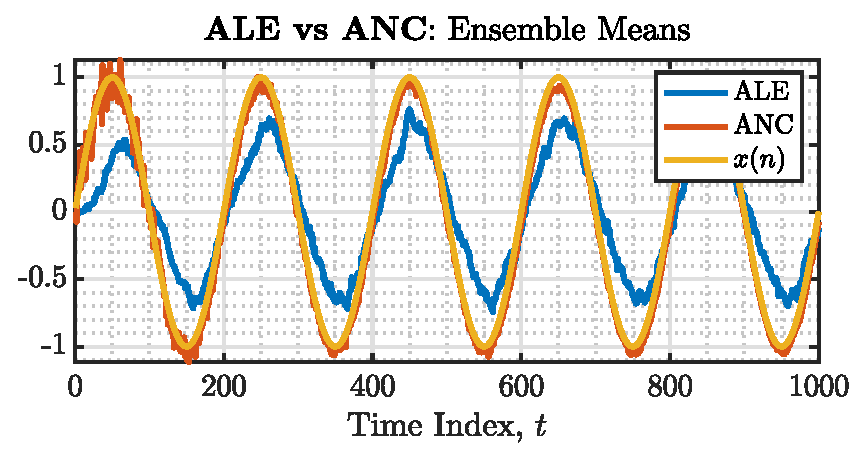
\includegraphics[height=1.5in]{report/adaptive-signal-processing/adaptive-noise-cancellation/assets/c/comparison}
    \end{subfigure}
    \caption{ALE vs ANC: ensemble mean comparison.}
    \label{fig:3_3_c_2}
\end{figure}

%% d)
\item
%

Let a synthetic reference input, $\epsilon(n)$, composed of a sinusoid of $50\ Hz$ corrupted by white Gaussian noise. The ANC configuration is used with inputs
$\epsilon(n)$ and the \texttt{POz} EEG time-series, in order to remove the strong $50 Hz$ frequency component due to power-line interference (mains).

For illustration purposes \texttt{spectrogram}s are plotted using a rectangular window of length $L=4096$ and $80\%$ overlap. The obtained spectrograms are provided
in figures \ref{fig:3_3_d_1} and \ref{fig:3_3_d_2}. As expected the original \texttt{POz} signal has a strong $50\ Hz$ frequency component.

\begin{figure}[h]
    \centering
    \begin{subfigure}{0.49\textwidth}
        \centering
        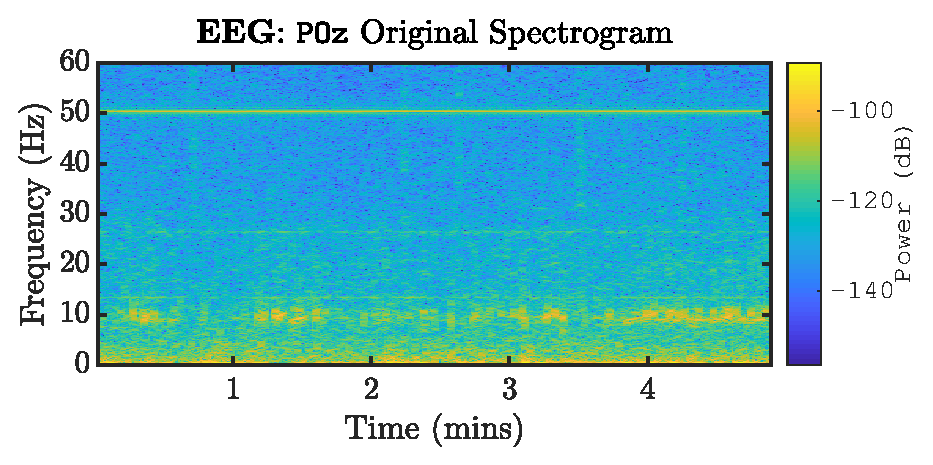
\includegraphics[height=1.5in]{report/adaptive-signal-processing/adaptive-noise-cancellation/assets/d/original}
    \end{subfigure}
    \caption{EEG: original, reference spectrogram.}
    \label{fig:3_3_d_1}
\end{figure}

The LMS filter order $M$ and the step-size $\mu$ is varied, and the impact on the spectrogram is shown in figure \ref{fig:3_3_d_2}.

\begin{figure}[h]
    \centering
    \begin{subfigure}{0.32\textwidth}
        \centering
        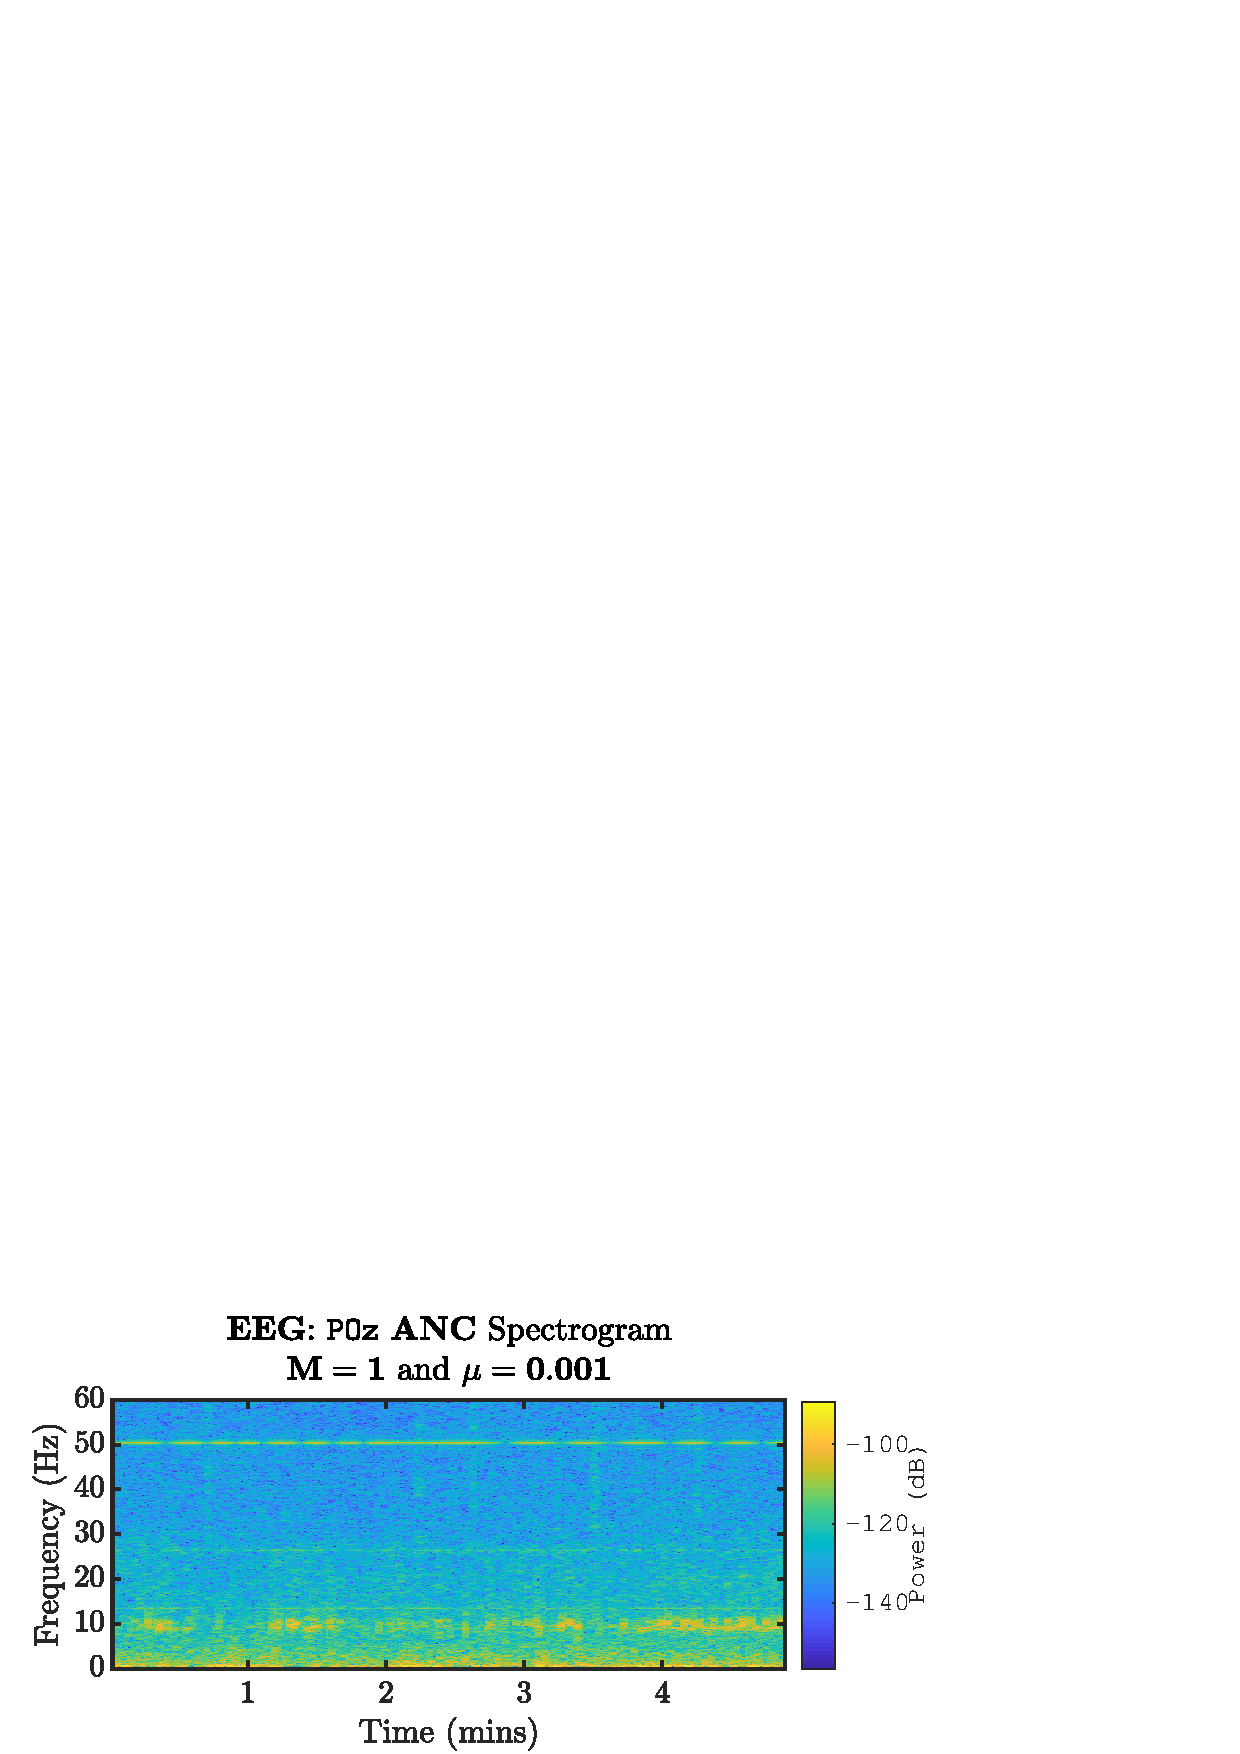
\includegraphics[height=1in]{{report/adaptive-signal-processing/adaptive-noise-cancellation/assets/d/M_1-mu_0.001}.pdf}
    \end{subfigure}
    ~ 
    \begin{subfigure}{0.32\textwidth}
        \centering
        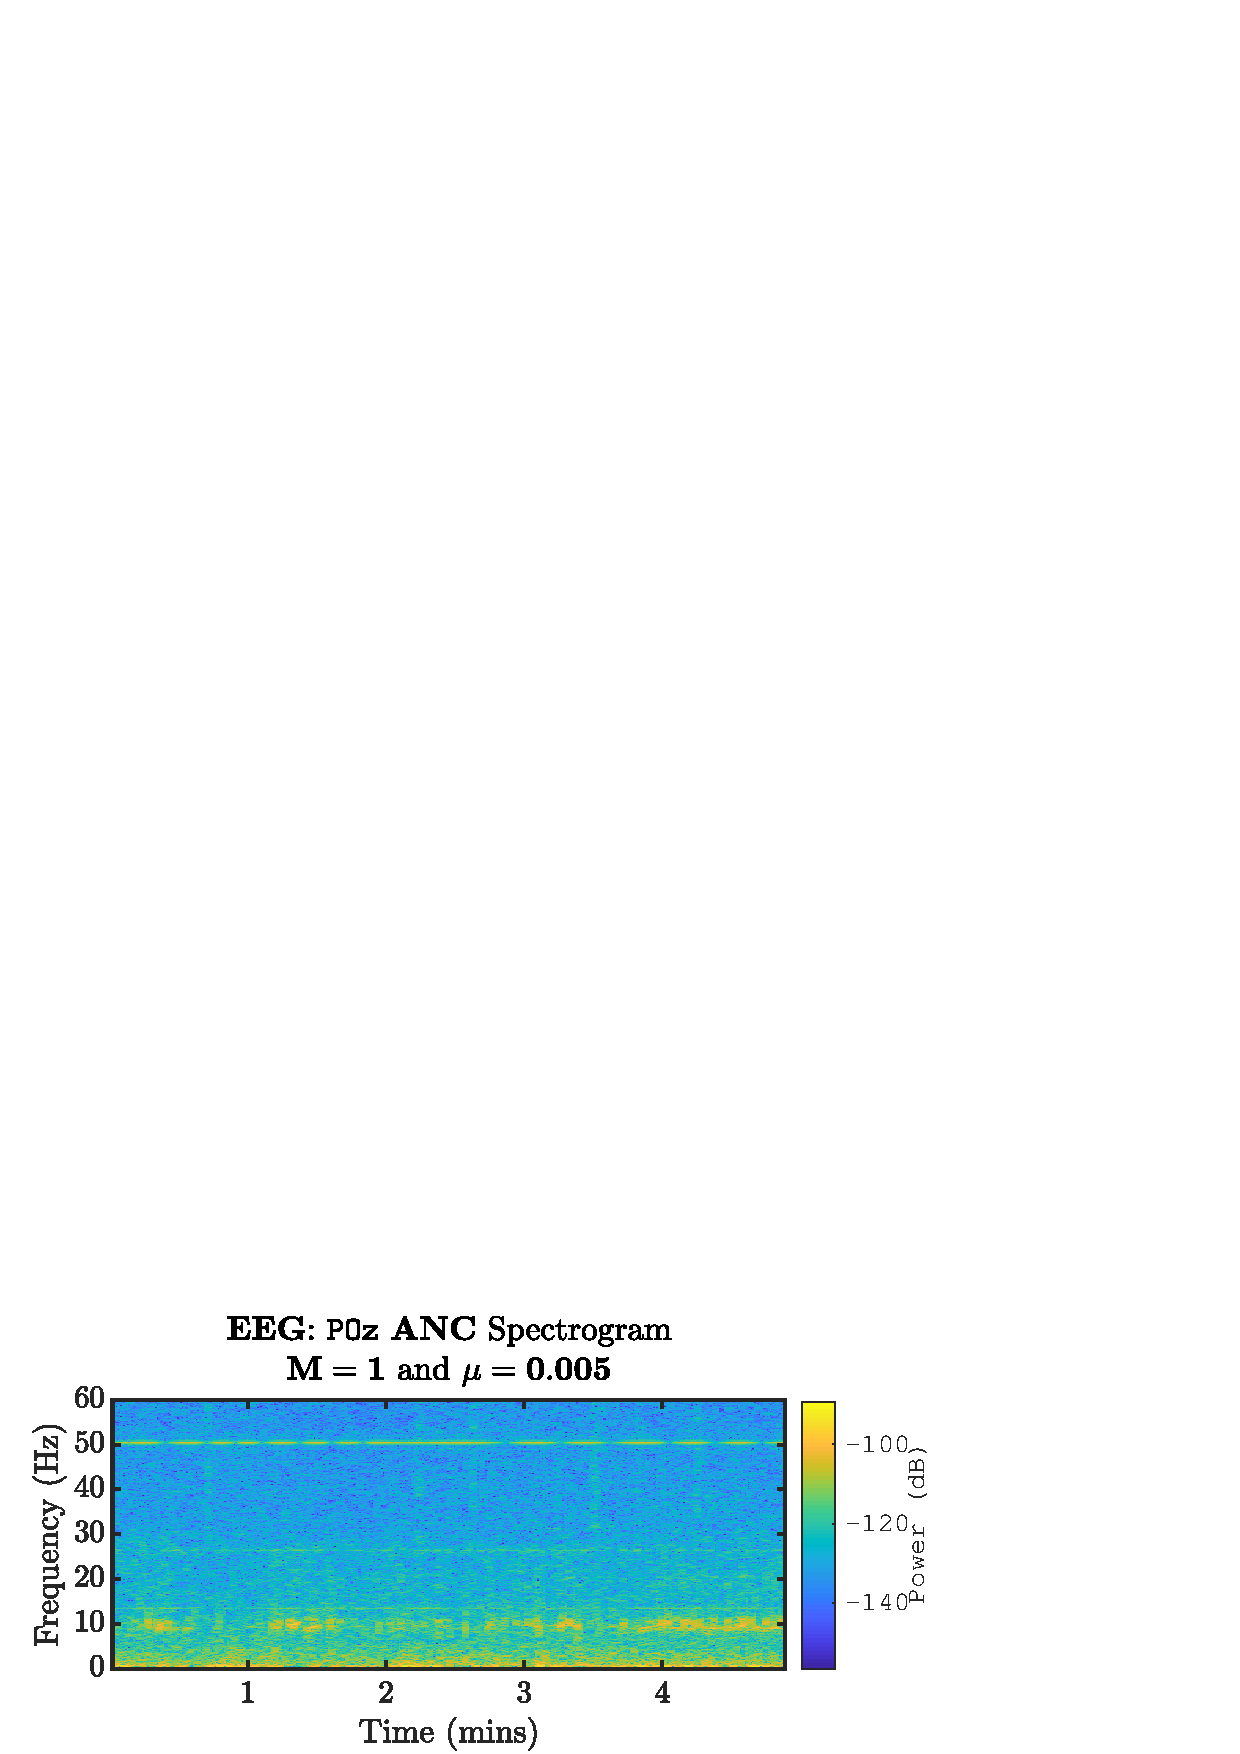
\includegraphics[height=1in]{{report/adaptive-signal-processing/adaptive-noise-cancellation/assets/d/M_1-mu_0.005}.pdf}
    \end{subfigure}
    ~
    \begin{subfigure}{0.32\textwidth}
        \centering
        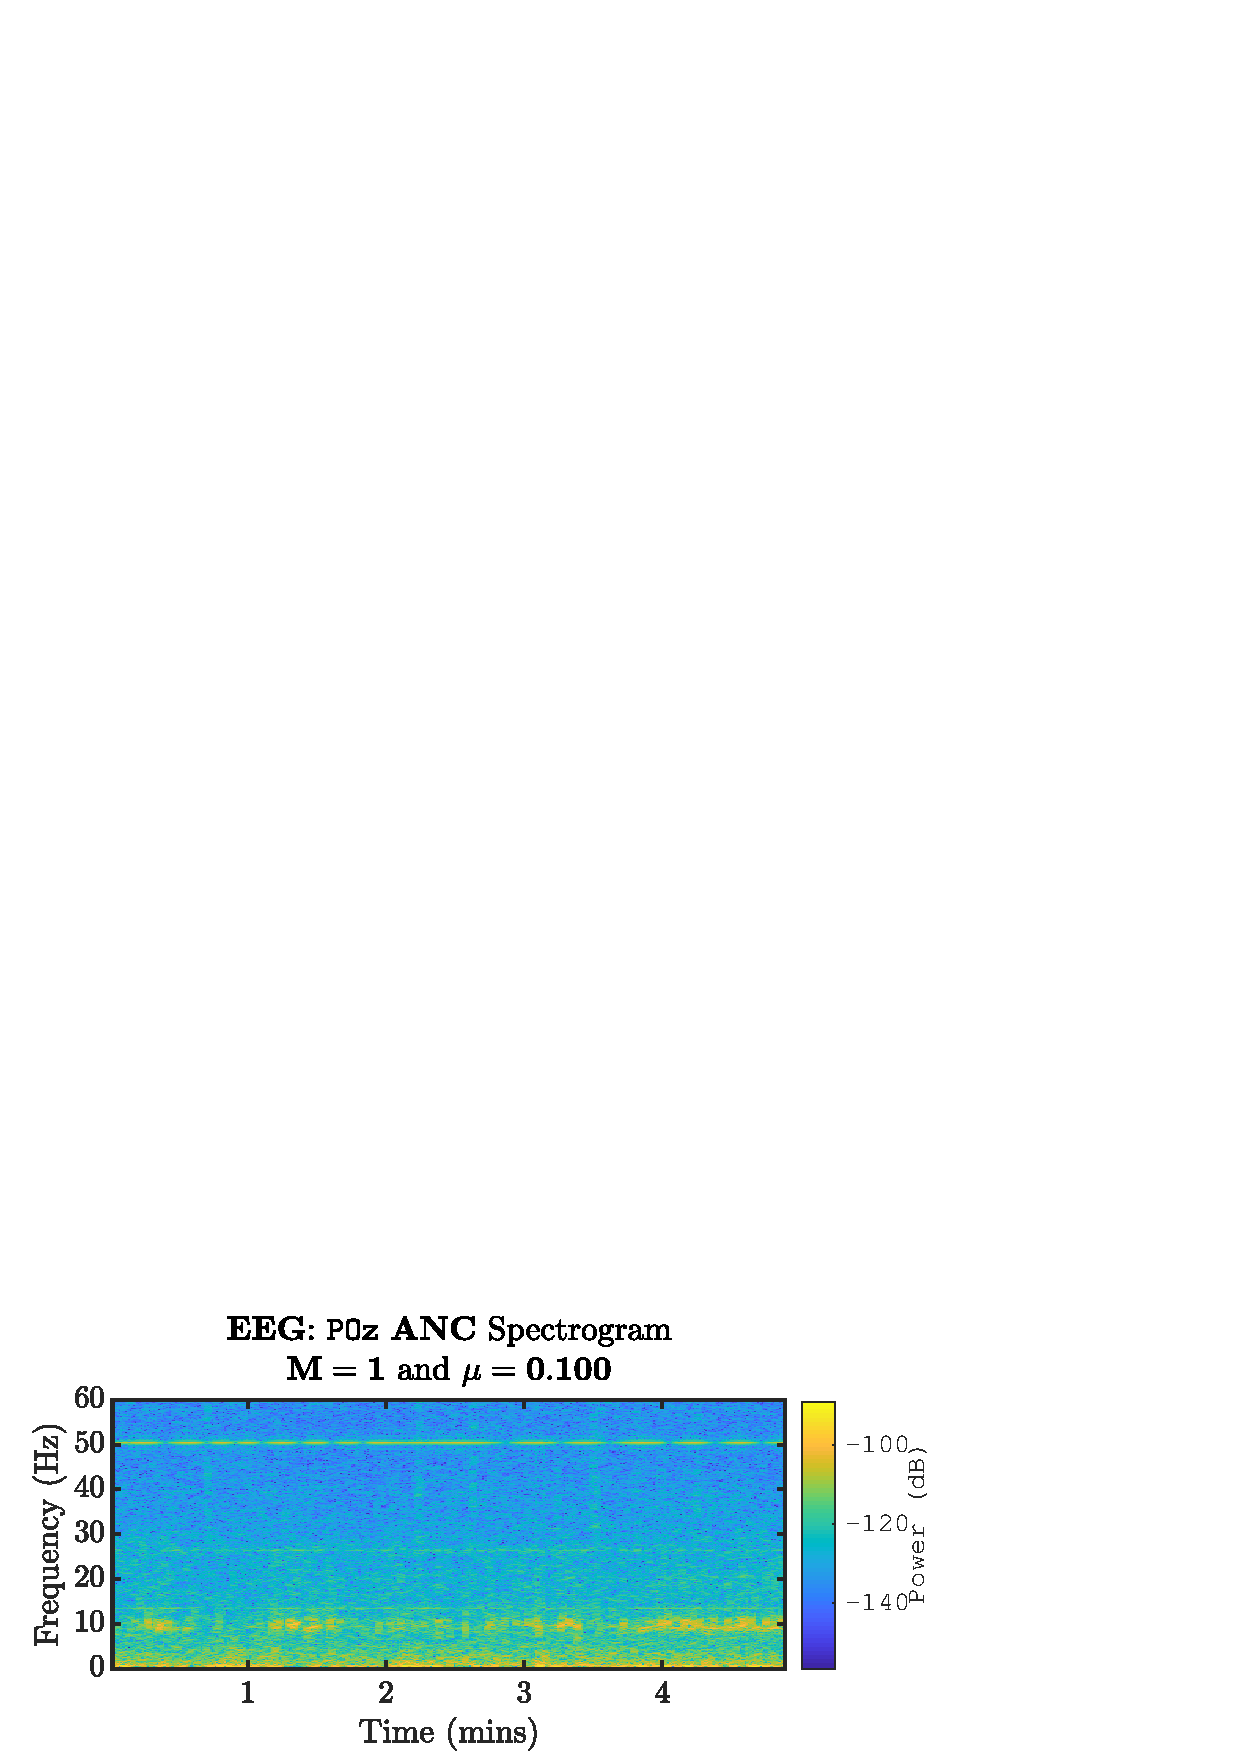
\includegraphics[height=1in]{{report/adaptive-signal-processing/adaptive-noise-cancellation/assets/d/M_1-mu_0.100}.pdf}
    \end{subfigure}
    ~
    ~
    \begin{subfigure}{0.32\textwidth}
        \centering
        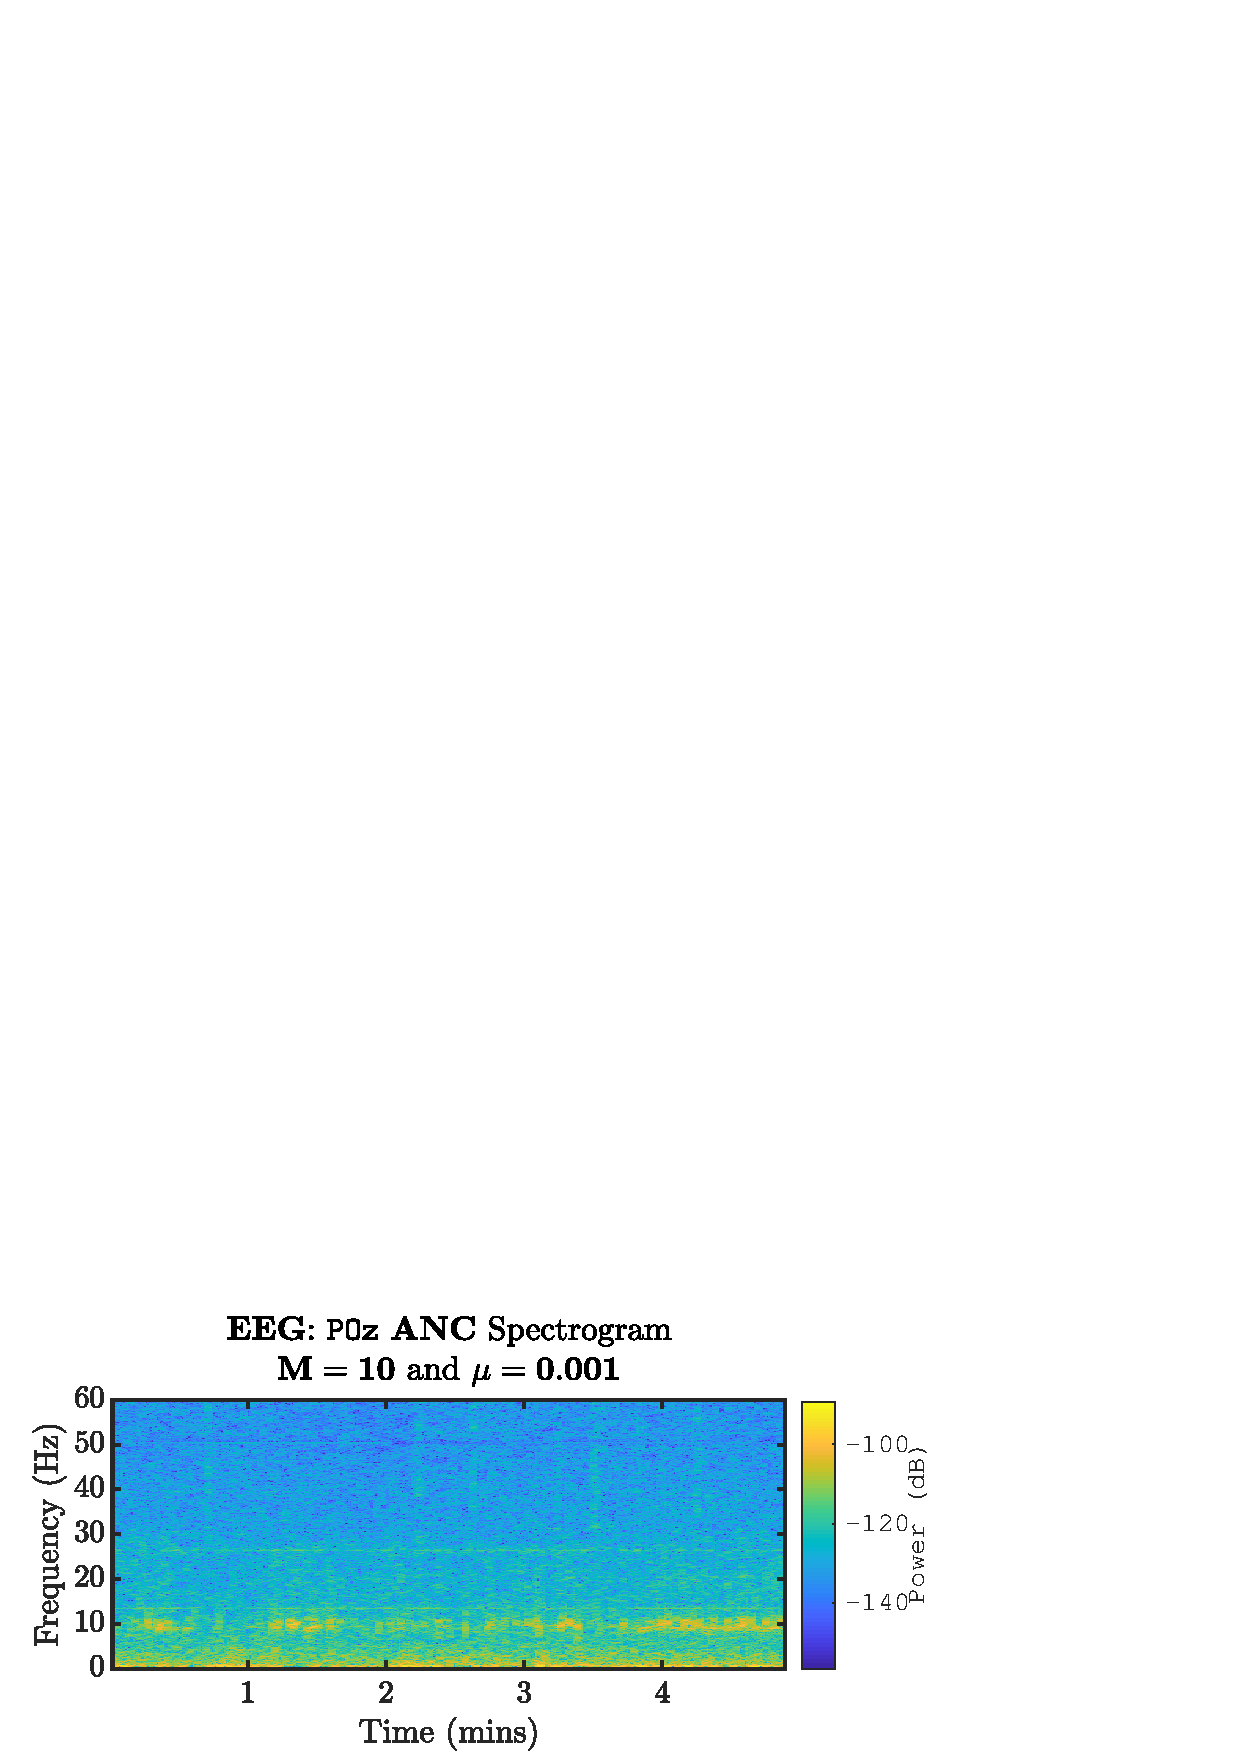
\includegraphics[height=1in]{{report/adaptive-signal-processing/adaptive-noise-cancellation/assets/d/M_10-mu_0.001}.pdf}
    \end{subfigure}
    ~ 
    \begin{subfigure}{0.32\textwidth}
        \centering
        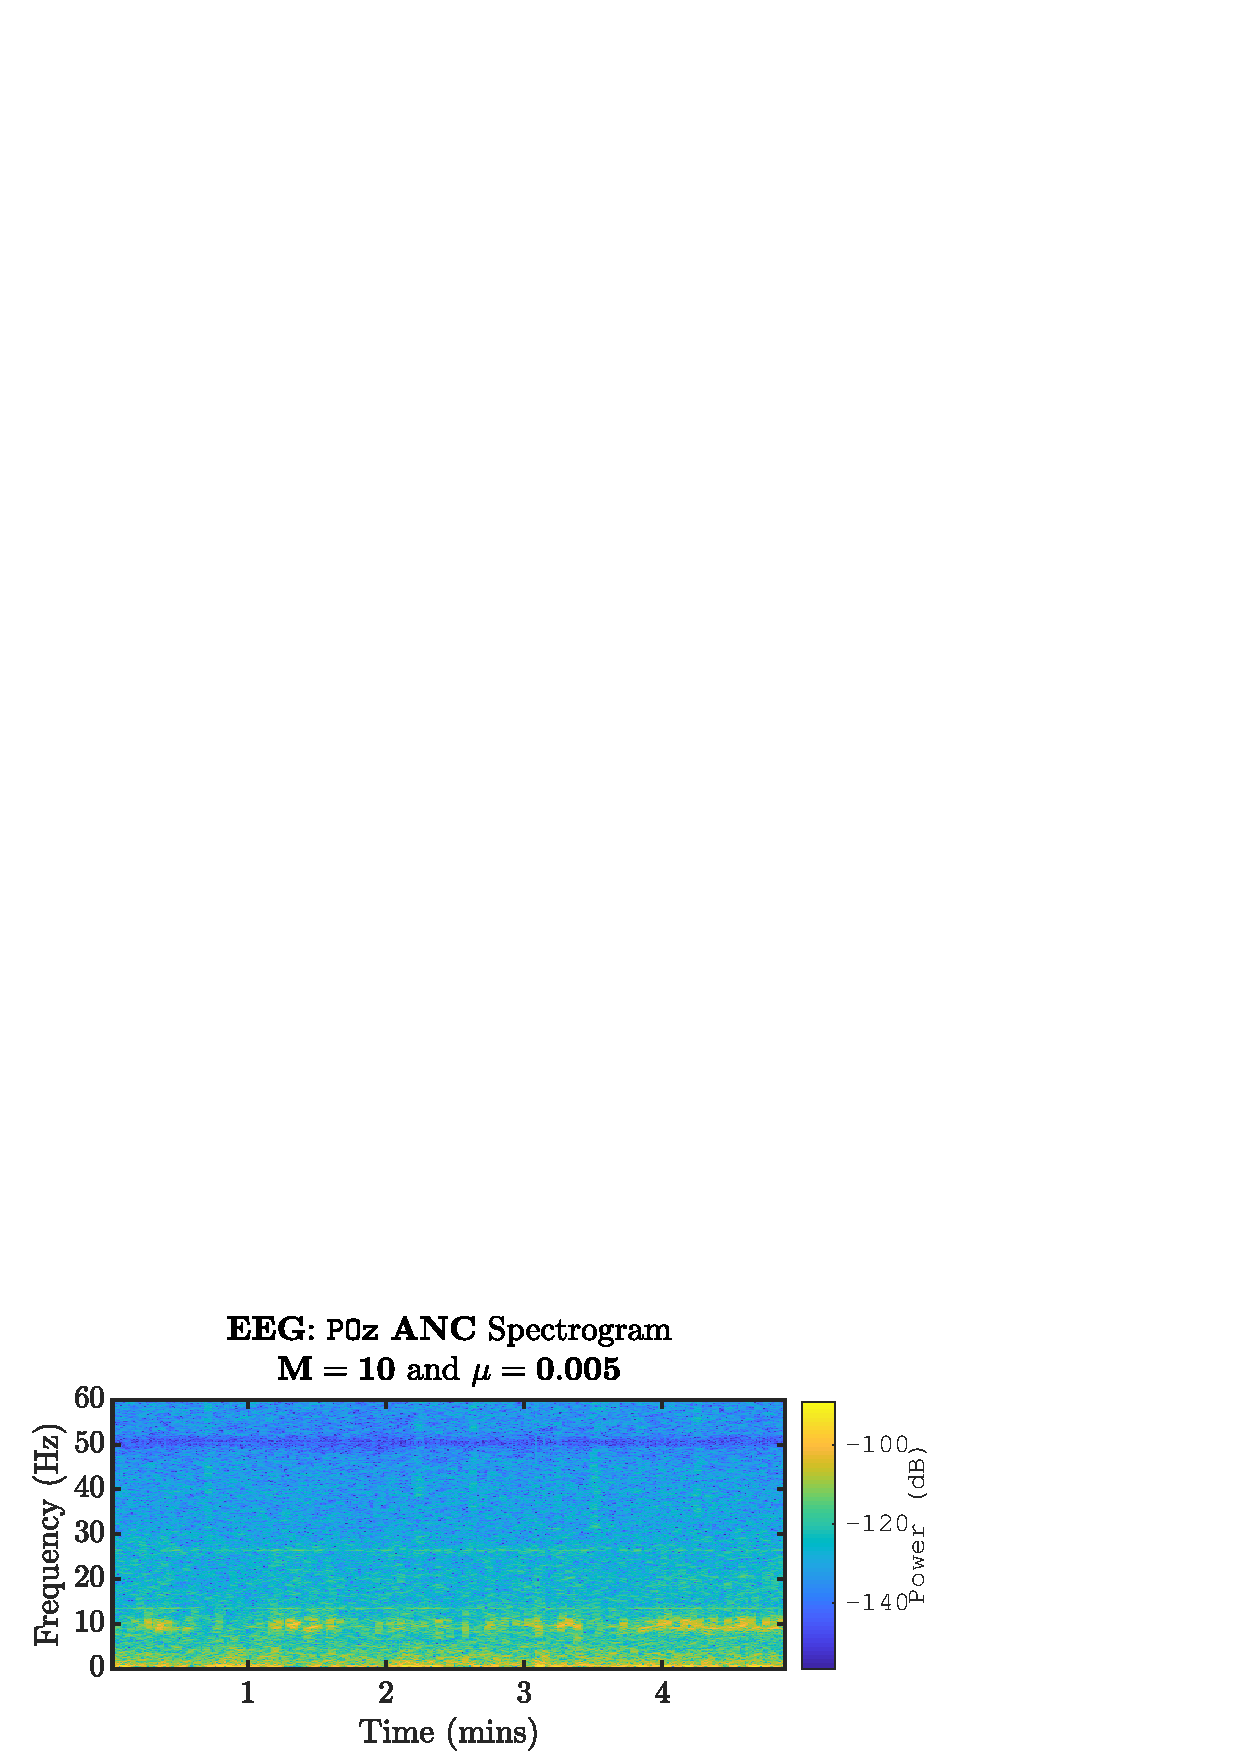
\includegraphics[height=1in]{{report/adaptive-signal-processing/adaptive-noise-cancellation/assets/d/M_10-mu_0.005}.pdf}
    \end{subfigure}
    ~
    \begin{subfigure}{0.32\textwidth}
        \centering
        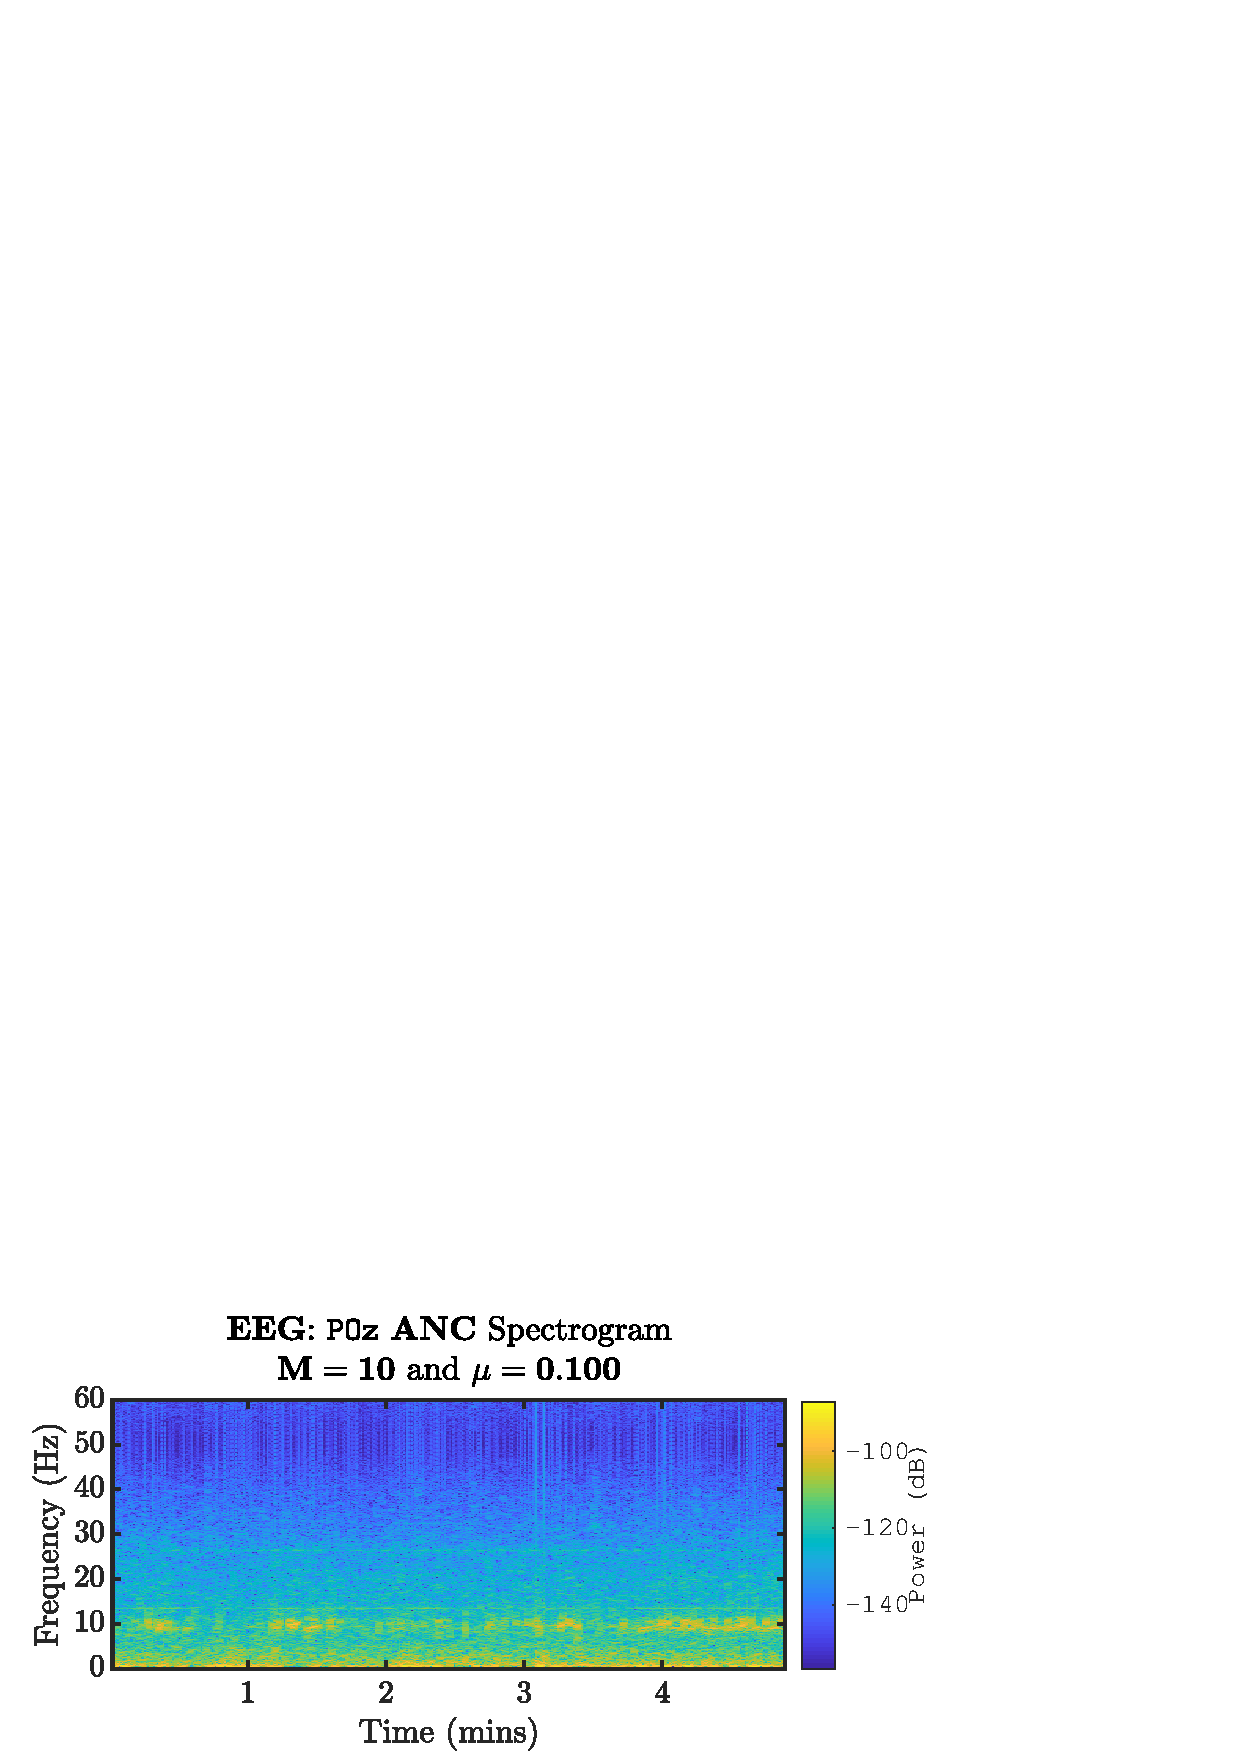
\includegraphics[height=1in]{{report/adaptive-signal-processing/adaptive-noise-cancellation/assets/d/M_10-mu_0.100}.pdf}
    \end{subfigure}
    ~
    ~
    \begin{subfigure}{0.32\textwidth}
        \centering
        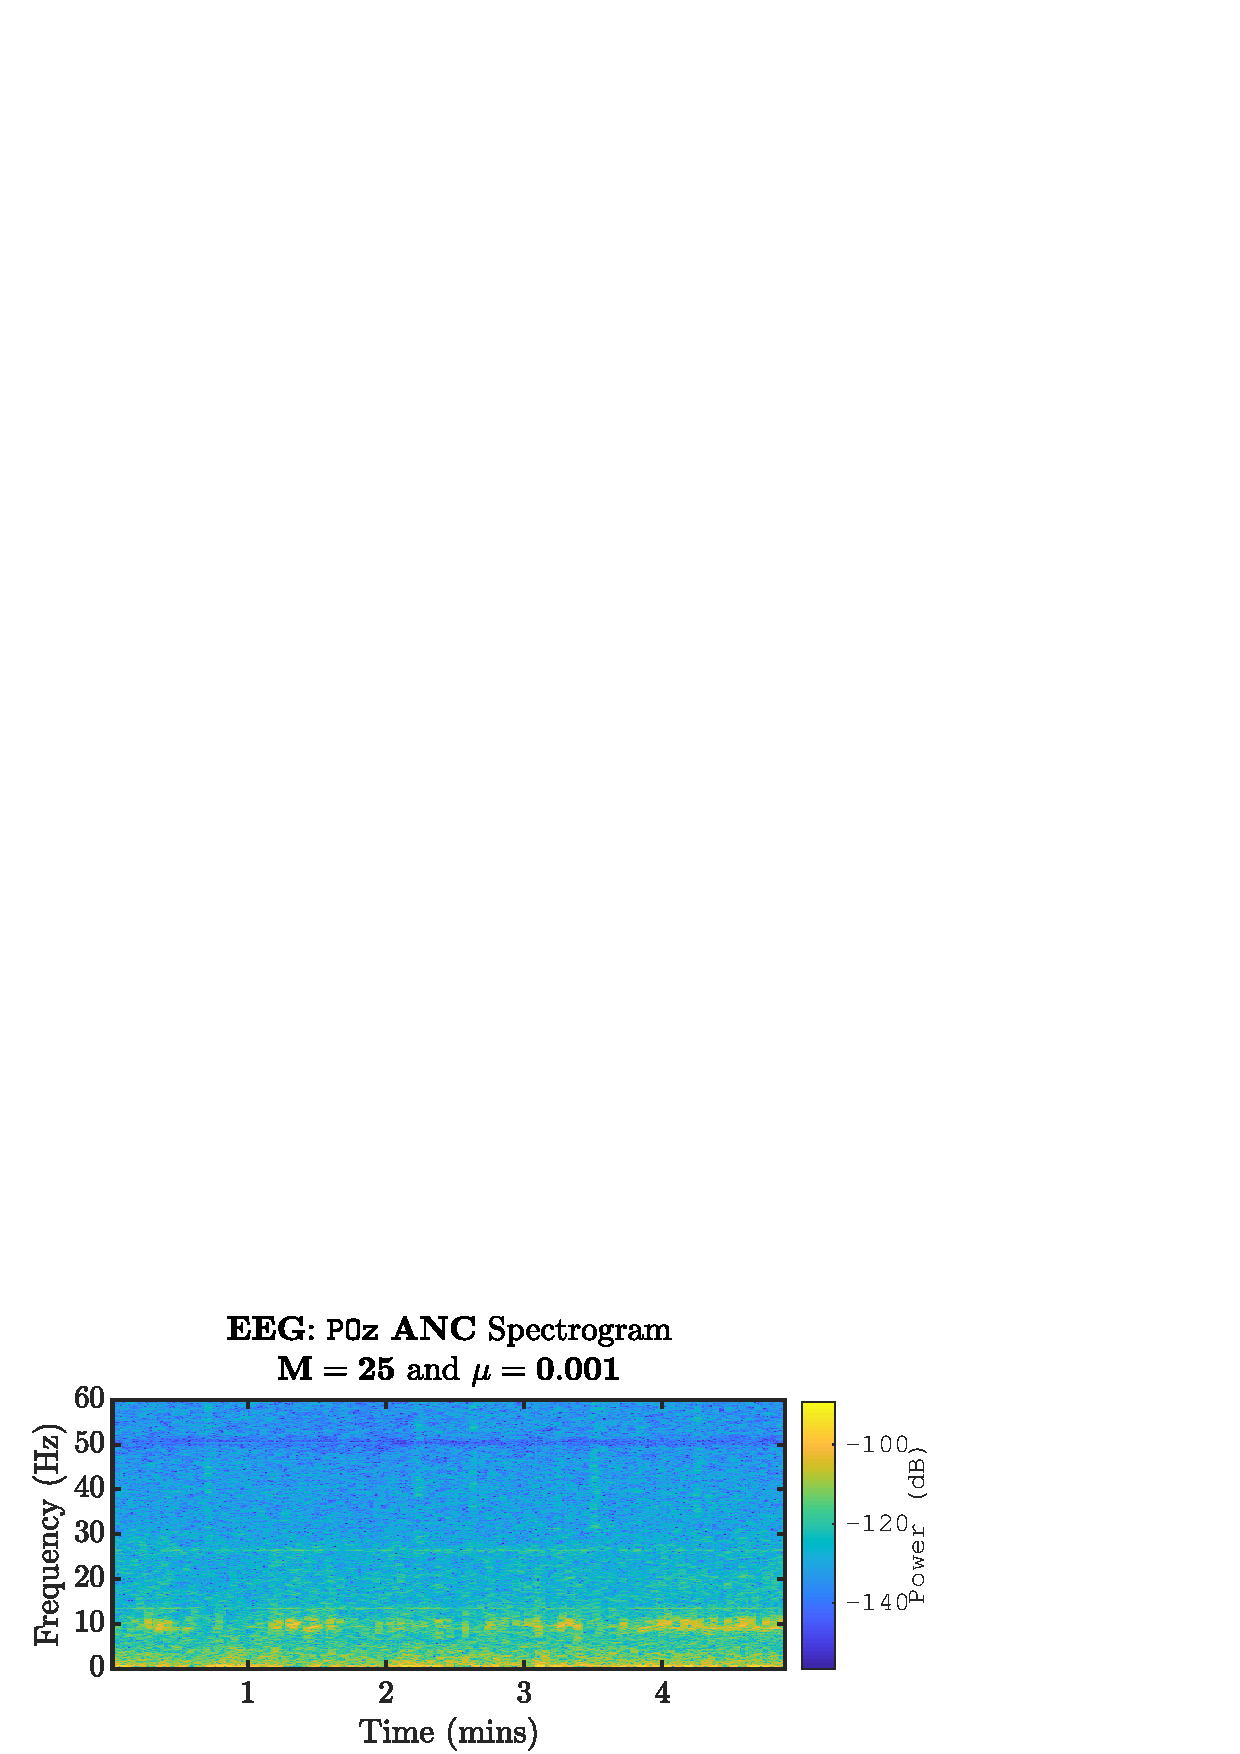
\includegraphics[height=1in]{{report/adaptive-signal-processing/adaptive-noise-cancellation/assets/d/M_25-mu_0.001}.pdf}
    \end{subfigure}
    ~ 
    \begin{subfigure}{0.32\textwidth}
        \centering
        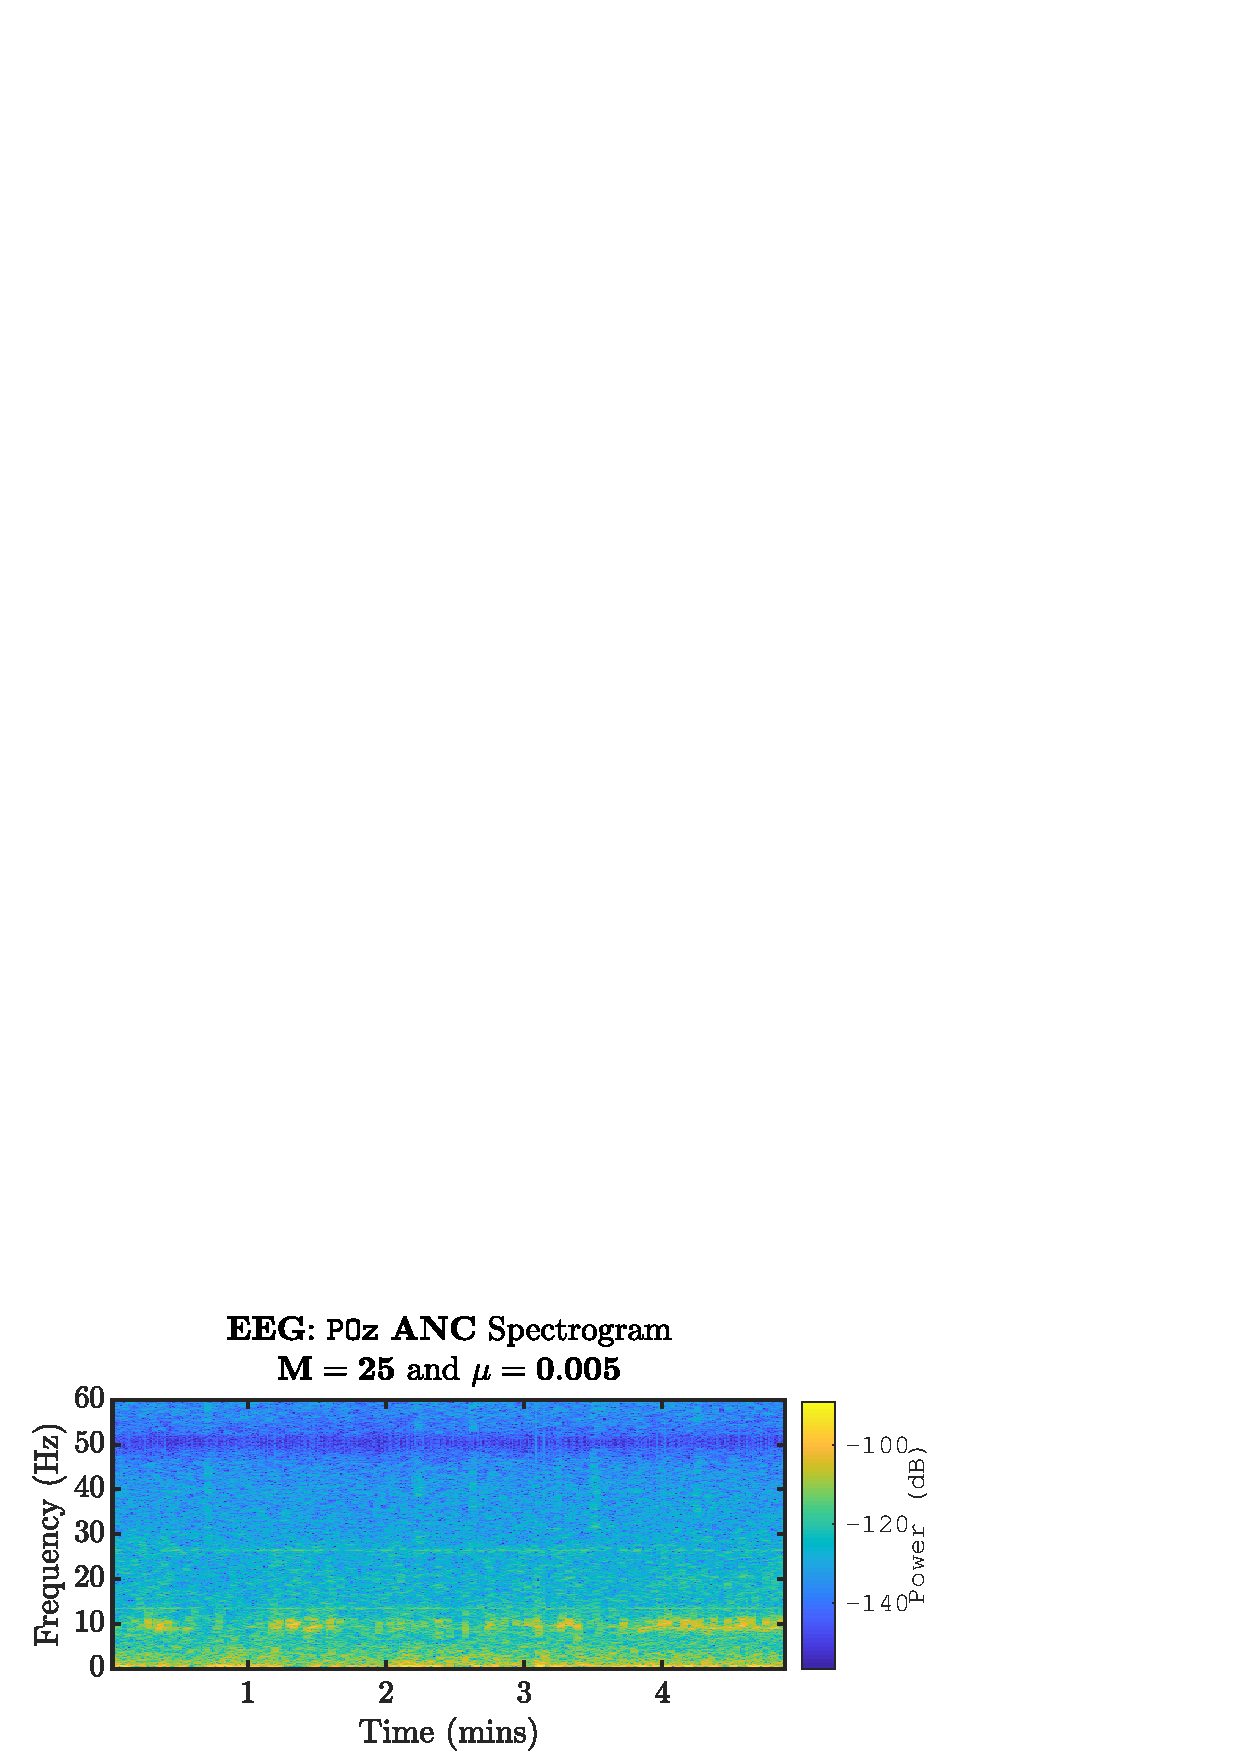
\includegraphics[height=1in]{{report/adaptive-signal-processing/adaptive-noise-cancellation/assets/d/M_25-mu_0.005}.pdf}
    \end{subfigure}
    ~
    \begin{subfigure}{0.32\textwidth}
        \centering
        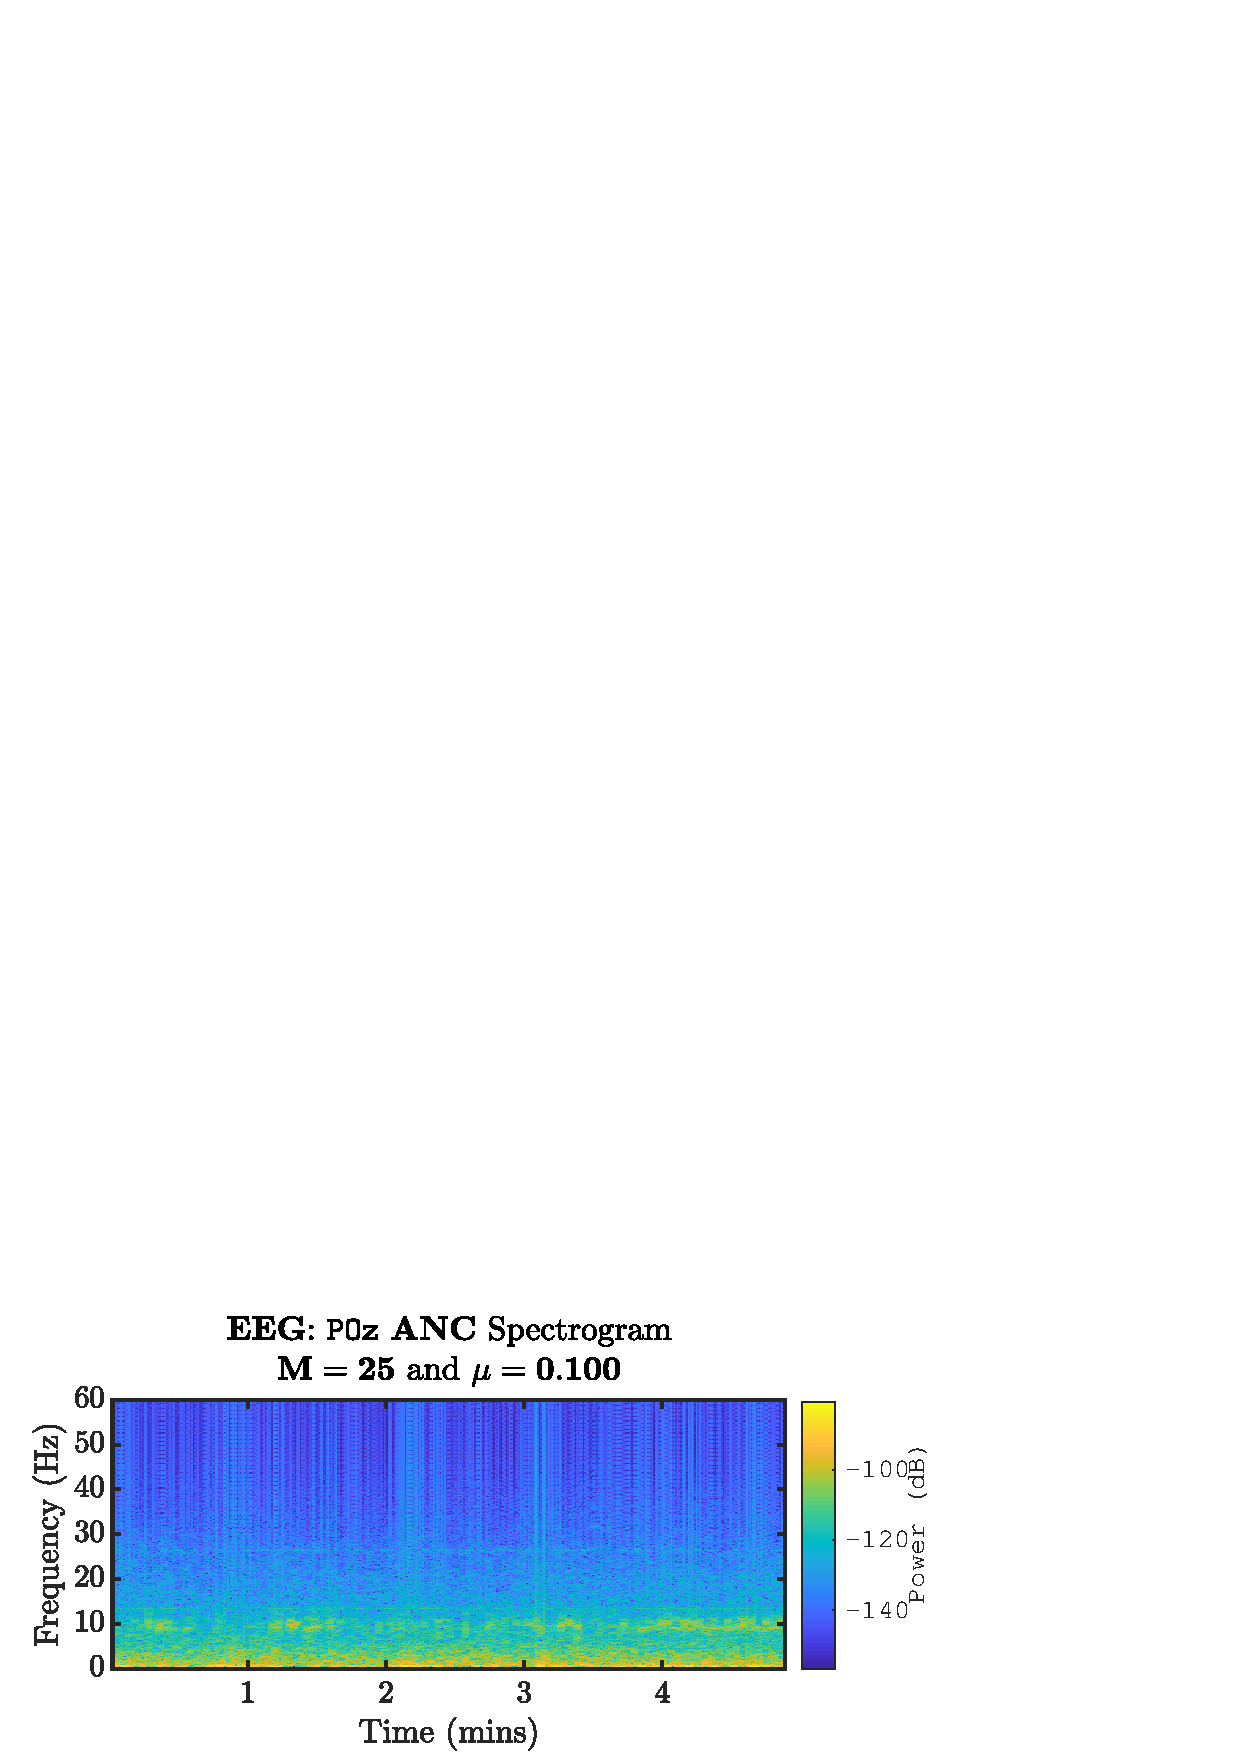
\includegraphics[height=1in]{{report/adaptive-signal-processing/adaptive-noise-cancellation/assets/d/M_25-mu_0.100}.pdf}
    \end{subfigure}
    \caption{EEG: ANC denoised spectrogram for different model order, $M$, and step-sizes, $\mu$.}
    \label{fig:3_3_d_2}
\end{figure}

Large step-sizes (i.e $\mu = 0.1$) affect significantly the spectral components around $50\ Hz$, degrading ANC performance.
On the other hand, small step-sizes (i.e $\mu = 0.001$) take more time to reach steady-state, however provide successful denoising, without disrupting the frequencies close to $50\ Hz$.

On the other hand, under-modelling (i.e $M = 1$) leads to poor noise cancellation, since the $50\ Hz$ power-line interface component has not been attenuated.
However, over-modelling (i.e $M=25$) degrades quality of neighbour frequencies, while a medium size model, such as $M=10$, achieves satisfying performance, by eliminating the
$50\ Hz$ component of interest, without affecting any other compoenents.

Overall, an ANC configuration with $(M, \mu) = (10, 0.001)$ is selected. The corresponding denoised periodogram is also provided at figure \ref{fig:3_3_d_3}.

\begin{figure}[h]
    \centering
    \begin{subfigure}{0.49\textwidth}
        \centering
        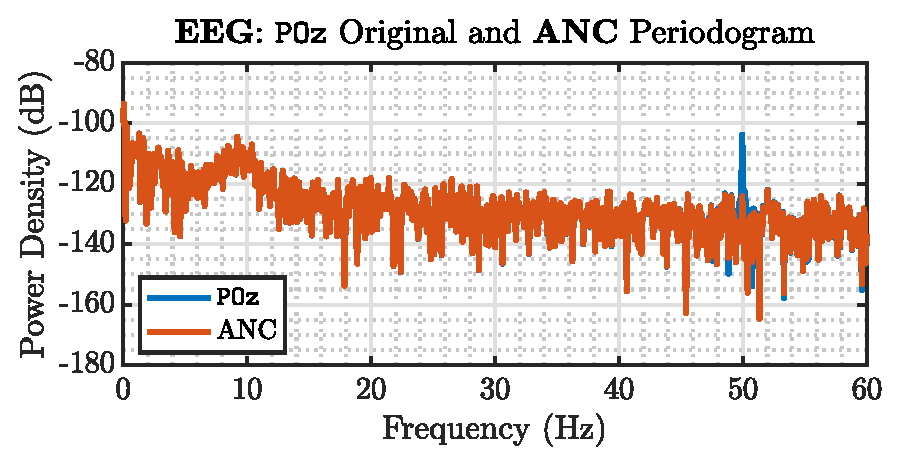
\includegraphics[height=1.5in]{report/adaptive-signal-processing/adaptive-noise-cancellation/assets/d/periodogram}
    \end{subfigure}
    ~
    \begin{subfigure}{0.49\textwidth}
        \centering
        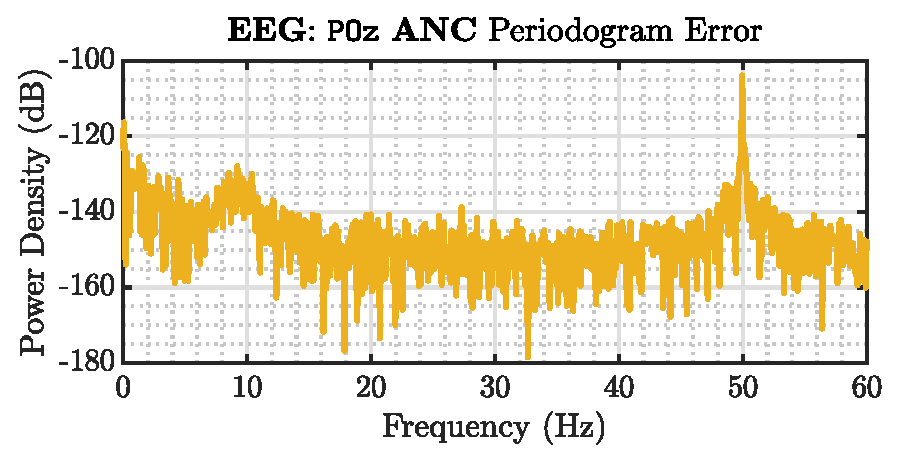
\includegraphics[height=1.5in]{report/adaptive-signal-processing/adaptive-noise-cancellation/assets/d/periodogram-error}
    \end{subfigure}
    \caption{EGG: periodograms of original and denoised signals.}
    \label{fig:3_3_d_3}
\end{figure}

%
\end{enumerate}